\chapter{Radar system overview}

In order to build a model capable of accurately capturing key features from various areas one must first understand the origin of the received signal. In this chapter a few fundamental concepts in radar systems are introduced considered critical for understanding the radar responses produced in the measurement setup outlined in the previous chapter. First, the basic principles of radar is explained. The manner in which electromagnetic waves disperse and scatter in a space are briefly discussed. Then, some important features in an actual radar system are considerd. These involve how the radar transmits its wavelets, the mixing process of returning waves and the demodulation procedure used for accurate phase tracking. 

\section{The radar principle}

The radar principle is at its core simple. A radar operates by radiating electromagnetic energy and analyzing returning echoes from reflecting targets in its field of view \citep{skolnik_2009}. By examining properties of the echo signal it is possible to obtain information about the targets. This may involve the range at which scatterers are located, the angles at which targets are found or the speed at which a scatterer moves \citep{richards_2014}. With a sufficiently high angular and range resolution it is possible to discern parts of the targets' size and shape. 

Radars are usually active systems, meaning that they have a radiating antenna and do not depend on ambient radiation \citep{skolnik_2009}. To perform measurements, a wavelet pulse $x_T(t)$ with some carrier frequency $\Omega$  is transmitted towards an object of interest. If a perfect reflector is present at distance $d$, the wavelet will return $2d/c$ seconds after transmission, where $c$ denotes the speed of light in air. Thus, the distance to a target object is calculated as 

\begin{equation}
	\label{eq:dist_time}
	d = \frac{ct}{2}.
\end{equation}

Note that we must divide by 2 in equation \ref{eq:dist_time} in order to accomodate for the pulse travelling back and forth (or, perhaps more accurately, forth and back) between the sensor and the scatterer. 

%After the previously transmitted wavelet is guaranteed to have died out, a new one is transmitted. Again, the radar listens for an echo, but this time after another time $t_2$ has passed. $t_2$ is greater than $t_1$, meaning the radar listens for echoes further away. If an echo is received, it means there is an object present at distance 

%$
%	d_2 = \frac12(c\cdot t_2).
%$
%This process is repeated for different time delays $t_i$. The chosen time delays can be adjusted depending on in what ranges one wants to search in, and how good range resolution one seeks. Together, the echoes (or lack thereof) from each transmitted wavelet make up what we call a \textit{sweep}. Before going through any preprocessing, a sweep can look like the one in figure \ref{fig:single_sweep_raw}.

%After a radar wavelet is transmitted and reflected on a single scatterer, it can be described mathematically as \citep{richards_2014}
%\begin{equation}
%	\label{eq:raw_sweep}
%	x_R(t)=A(t)\sin(\Omega t +\theta (t)),
%\end{equation}
%where $t$ relates to distance according to equation \eqref{eq:dist_time}. The major part of the receiver processing consists of extracting $A(t)$ and $\theta(t)$ explicitly from \eqref{eq:raw_sweep}. This process, known as quadrature demodulation, is described in appendix... and the benefits of doing this is further discussed in chapter \ref{IQ}.

\begin{figure}[h]
	\centering
	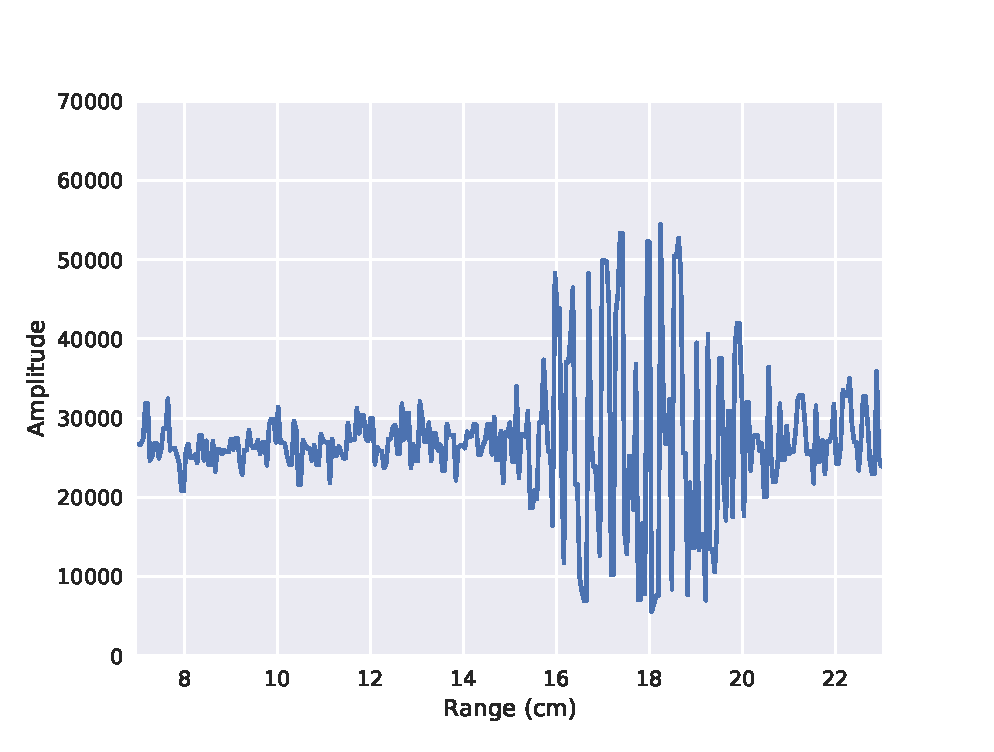
\includegraphics[scale=0.7]{figs_temp/single_sweep_raw}
	\caption{A single radar sweep which has been measured from 7 to 23 cm. The largest amplitude at around 18 cm. suggests there is some object present at that distance from the sensor.}
	\label{fig:single_sweep_raw}
\end{figure}

%\subsection{Radar wave dispersion}
%The transmitted signal from a radar is typically in the shape of a cone. Although, to understand how the signal propagates in space and develops over time, it helps to imagine that the signal is transmitted isotropically in a spherical manner.

%Assuming a signal with power $P_t$ is transmitted isotropically in a medium where no power is lost, the power density at range $R$ will be the total signal power divided by the surface area of a sphere with radius $R$. That is, $\rho_{t,R} = P_t/(4\pi R^2)$.

%How signals get weaker by a factor 1/r4


%1-dimensional data: signals propagate in a spherical manner

%How this ties in to what we do


%If it is assumed that the radar pulses are transmitted isotropically, and no power is lost in the transmission medium, the power density at a range $R$ is the emission power $P_t$ divided by the surface area of a sphere with radius $R$.

%The ratio $R$ between the transmitted signal power nd the received signal power is described in the \emph{Radar Transmission Equation}, seen below. Relating the 

%In this report a singular radar transmitter and receiver is used. 



%\citep{skolnik_2009}, \citep{richards_2014}


%\section{Radar operation}

%A pulsed radar system can be realized in countless ways, but all subscribe to the fundamental physical laws of electromagnetic radiation. In this section one such configuration is described. Furthermore, we describe the key signal processing method, \emph{In-phase and Quadrature-phase demodulation} (IQ demodulation), used for extracting useful information from the unprocessed radar response. 

%\subsection{Elements of a pulsed radar}
%The radar system considered in this report includes the following crucial components:

%\begin{itemize}
%	\item Waveform generator
%	\item Oscillator
%	\item Transmitting antenna
%	\item Receiving antenna
%	\item Mixer
%	\item Integrator
%\end{itemize}

% List of parts in radar system
% Nice figure showing this process


%A waveform generator outputs a radar envelope which is modulated by a local oscillator to some desired radio frequency. After signal amplification the wavelet is transmitted through an antenna. Detection is performed by a second antenna, which receives the returning signal during some time interval. 

\subsection{Mixing}


If a transmitted wavelet of angular frequency $\Omega$ is transmitted towards a single scatterer, the returning signal can be modeled as

\begin{equation}
	r(t) = A(t)\sin(\Omega t + \theta(t)).
\end{equation}

where $A(t)$ represents the pulse envelope. $r(t)$ is measured by elementwise multiplication of an internally generated reference signal $s(t)$.  

% MIXING PROCESS HERE

In this work we are investigating moving targets, which renders doppler frequency shifts in the echo waveform. Thus we are primarily interested in detecting veclocity components in $r(t)$, which shows up in the $\theta(t)$ function. Effective tracking of the $\theta(t)$ function can be achieved through \emph{IQ demodulation}. 


Our target is to find $\theta(t)$, providing information about the target scatterer.  




%We previously stated that after the radar has transmitted a pulse, it listens for an echo. This process is more formally called \textit{mixing}. After having transmitted a pulse, an internal wavelet is generated at a very specific delay from the initial pulse transmission. This internal wavelet is multiplied with the received signal. If the received and internal pulses do not match, the output of this multiplication will be zero. If there however exist some overlap between the internal and returning signals the output will be nonzero, indicating some level of energy content at the distance corresponding to the internal pulse delay. By increasing the internal pulse delay and repeating this procedure a set of measurement points is obtained. Mixing is thus achieved by multiplying a large number of returning wavelets with internally generated wavelet counterparts, adding a slight delay between sampling points. 

% Describe why this process is equivalent to an autocorrelation
% Include plot of raw data to show what a real sweep looks like.

%Figures \ref{fig:mix0}, \ref{fig:mix1} and \ref{fig:mix2} illustrate this principle. In the upper plot in the first two figures two analysis wavelets are shown, each at a different time delay. The center plot show the received radar pulse registrered by the antenna, and the lower plot the result when the two above signals are multiplied elementwise. Note that the final figure show the result of multiple received electromagnetic pulses, each sample point representing a summation of one set of multiplications between returning and internally generated signals. This output will henceforth be called the \emph{raw signal}.   

\begin{figure}[h]
	\centering
	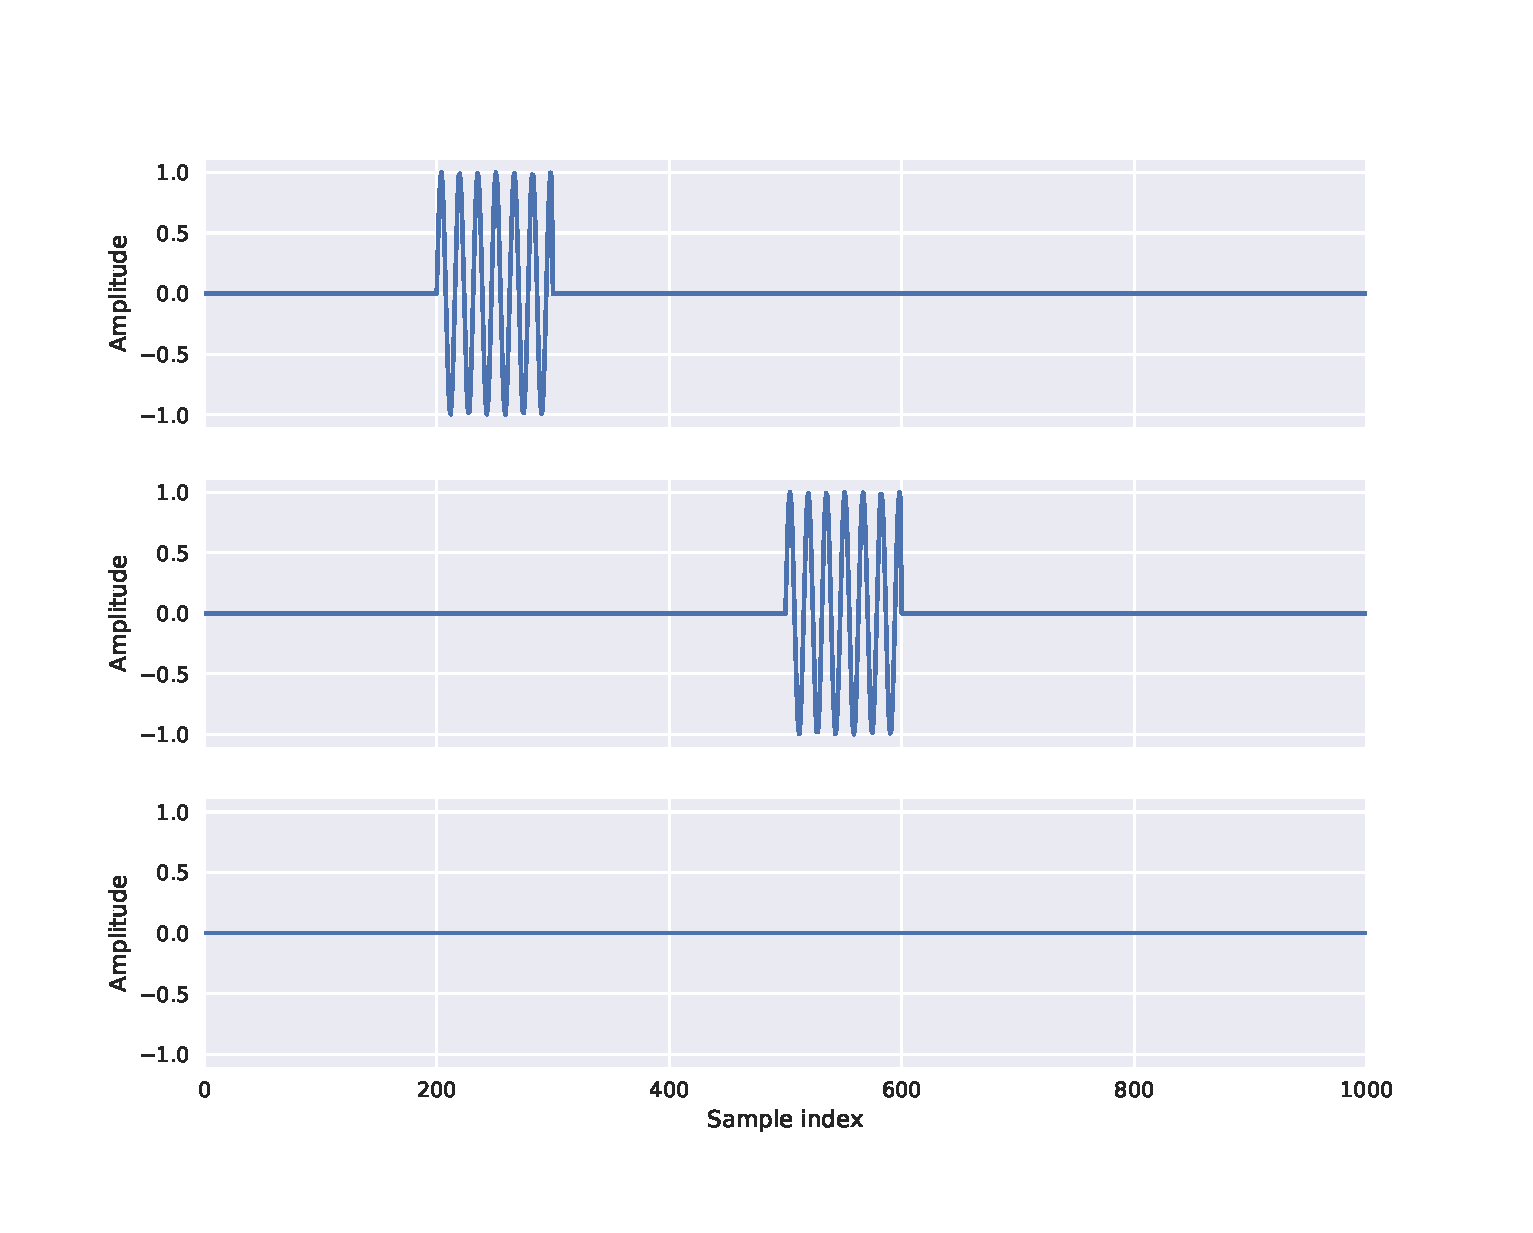
\includegraphics[scale=0.5]{figs_temp/mixing0}
	\caption{Analysis pulse (top), received pulse (mid) and multiplication output (bot). As the signals do not overlap the multiplication yields only zero values.}
	\label{fig:mix0}
\end{figure}

\begin{figure}[h]
	\centering
	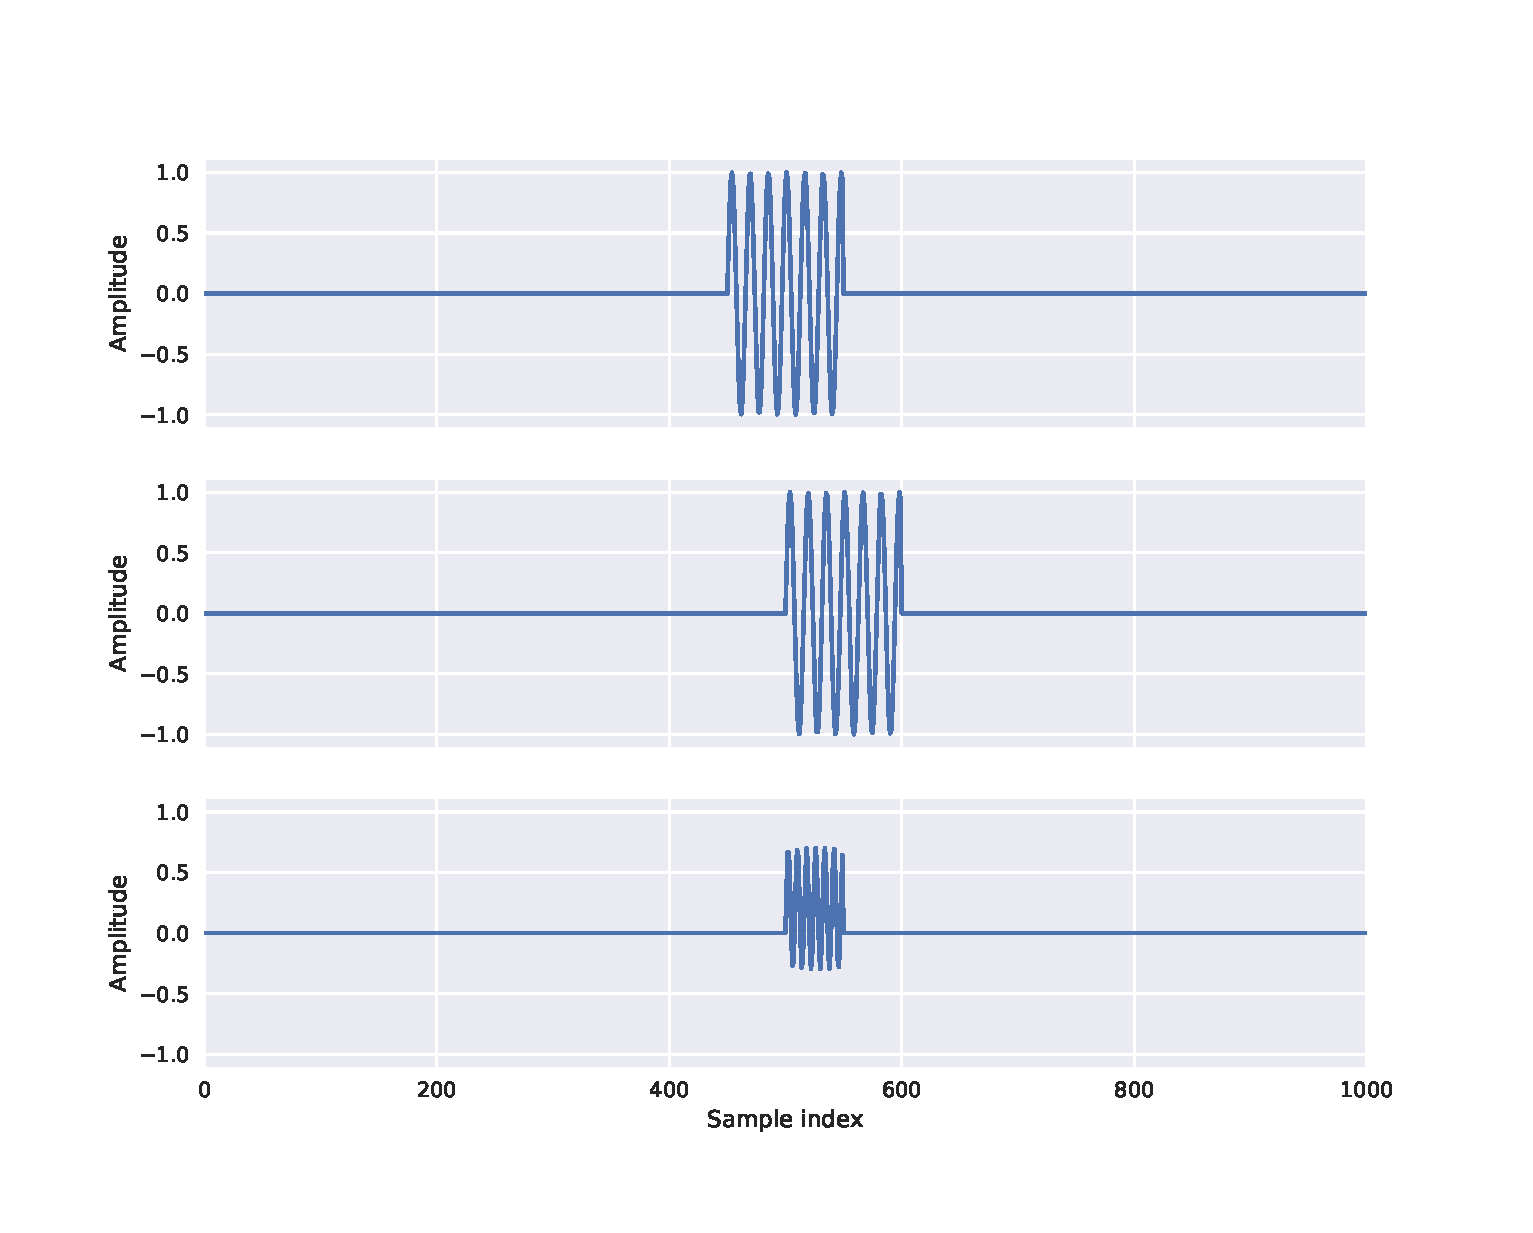
\includegraphics[scale=0.5]{figs_temp/mixing1}
	\caption{Analysis pulse (top), received pulse (mid) and multiplication output (bot). The overlapping signals produce varying amplitudes at the output sensitive to small changes in phase.}
	\label{fig:mix1}
\end{figure}

\begin{figure}[h]
	\centering
	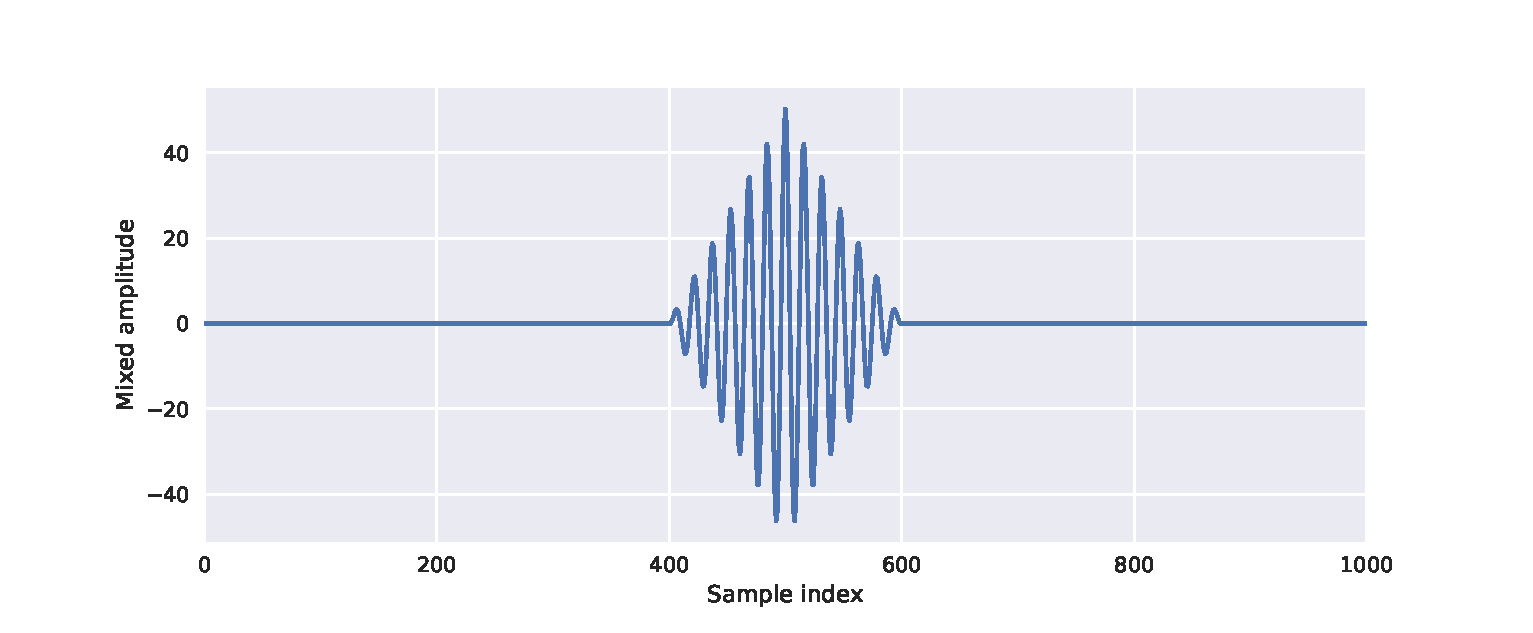
\includegraphics[scale=0.5]{figs_temp/mixing2}
	\caption{By integrating the multiplication at each delay the mixing output is produced.}
	\label{fig:mix2}
\end{figure}



%\subsection{IQ demodulated data}
%\label{IQ}
%A common type of data when working with radar signal processing is in-phase and quadrature-phase data (IQ-data). IQ-data is represented as complex numbers, and a radar sweep consists of several such complex numbers - one for each investigated range. The process of obtaining IQ-data is often referred to as IQ- or quadrature demodulation, and is described in appendix .... The usefulness of this type of data lies in that it contains explicit information about the amplitude, $A(t)$, and phase, $\theta(t)$, in equation \eqref{eq:raw_sweep} \citep{richards_2014}. To obtain the amplitude for a sweep, $s$, one simply computes the absolute value for each complex number in $s$. The amplitude plot is a good way to visualize at what ranges objects are present. Figure \ref{fig:single_sweep_iq} illustrates such a graph where the same measurement setup as in figure \ref{fig:single_sweep_raw} has been used. Similarly, a phase curve can be obtained by computing the phase in each point.

%In many applications, the phase information in IQ-data is used when small changes in the radar signal need to be detected, (Mention a case such as recording over grass...) as the phase is more sensitive to changes than the amplitude \citep{lien_gillian_karagozler_amihood_schwesig_olson_raja_poupyrev_2016}. If an object is detected at distance $r(t_1)$ from the radar at time $t_1$, and shortly thereafter, the object is moved to distance $r(t_2)$, the corresponding difference in phase will be
%\begin{equation}
%	\label{eq:phase_diff}
%	\Delta\phi(t_1, t_2)=\frac{4\pi}{\lambda}(r(t_2)-r(t_1)) \quad\quad \textrm{mod 2$\pi$}
%\end{equation}
%By having a sampling frequency which is too low, the range difference in $\eqref{eq:phase_diff}$ could potentially become very big, and the phase difference would fluctuate over time and be incomprehensible.

%In the case of material classification, a high sampling frequency is highly beneficial. When moving across surfaces characterized by tiny details, a high sampling frequency is essential in capturing the shapes of these.

%\begin{figure}[h]
%	\centering
%	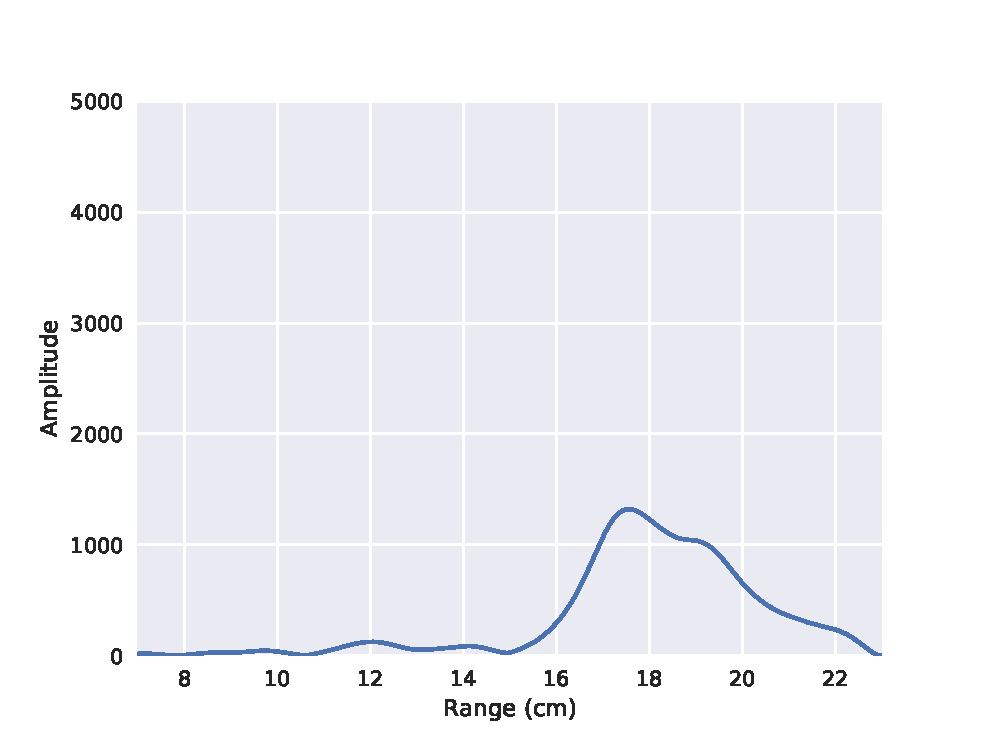
\includegraphics[scale=0.7]{figs_temp/single_sweep_iq}
%	\caption{Visualization of an amplitude function derived from IQ-data.}
%	\label{fig:single_sweep_iq}
%\end{figure}

%For a thorough description of how IQ-data is derived, see appendix ...











%
%

